\chapter{Deseño}

Neste capítulo documentarase o proceso de deseño que se irá formando de xeito incremental nas sucesivas iteracións da metodoloxía Scrum. Comentarase a arquitectura do modelo de datos que vai manexar a aplicación, así como a distribución deses datos na aplicación, o que nos obrigará a falar da interface gráfica de usuario. Despois disto, mergullarémonos no que é o deseño e máis a implementación dos compoñentes da aplicación.

\section{Estrutura do deseño}

Os datos son o punto de partida de todas as funcionalidades deste proxecto. Todo xira arredor do arquivo con información que o usuario importa tras abrir por primeira vez o JDataMotion. O dato debe ser almacenado de xeito adecuado, e accedido só a través dos métodos e clases necesarios, para manter o fluxo de información controlado. A clase que captará, almacenará e distribuirá os datos de cara ás demais clases da aplicación recibirá o nome de Modelo, posto que realmente alberga o modelo da aplicación.

JDataMotion vai ser un programa moi dependente da súa interface de usuario. Os diagramas de dispersión non poden ser visualizados a través dunha simple terminal, e o constante fluxo de datos entre o usuario e o sistema non se pode activar a través dun menú de opcións en termos de usabilidade. Si traballamos co JDataMotion a través dunha interface gráfica multifío como as que Java permite deseñar, a aplicación pode procesar a información ao mesmo tempo que o usuario realiza outras interaccións (ver o modelo, configurar un filtro ou mesmo cancelar a visualización dinámica). Por isto, a clase Vista será un dos artefactos que máis tempo adicaremos a implementar. Vista conterá os ``widgets'' da libraría Swing necesarios para presentar a información ao usuario, e recibir del as novas ordes. Será unha clase complexa e de bastante peso que delegará certas funcións en clases internas ou asociadas.

Só falta unha clase que reciba da Vista as funcionalidades activadas polo usuario e cree un comando que se encargue de realizar o traballo. Esta clase deberá non só disparar o comando, se non que tamén terá que xestionalo, e reaccionar dun xeito específico en caso de que o comando chegue a unha situación de erro. A maioría de comandos influirá directa ou indirectamente sobre o Modelo. A esta clase chamarémoslle Controlador porque a súa responsabilidade será esencialmente esa, a de recibir eventos da Vista e xestionar comandos que actúen de cara ao Modelo. Deste xeito a Vista utilizará a API do Controlador, e quedará exenta de responsabilidade no caso de que se detecten fallas no Modelo.

Acabamos de definir dun xeito explícito cal é o patrón de deseño sobre o que vai xirar toda esta fase do proxecto: o Modelo-Vista-Controlador (MVC). Os patróns de deseño son solucións prácticas a problemas de deseño comúns. En concreto, o Modelo-Vista-Controlador divide o sistema en tres compoñentes coas responsabilidades definidas que xa comentamos anteriormente. A mellor forma de expoñer a aplicación exacta do patrón MVC no noso proxecto é o diagrama da figura \ref{MVC}.

\begin{figure}
\centering
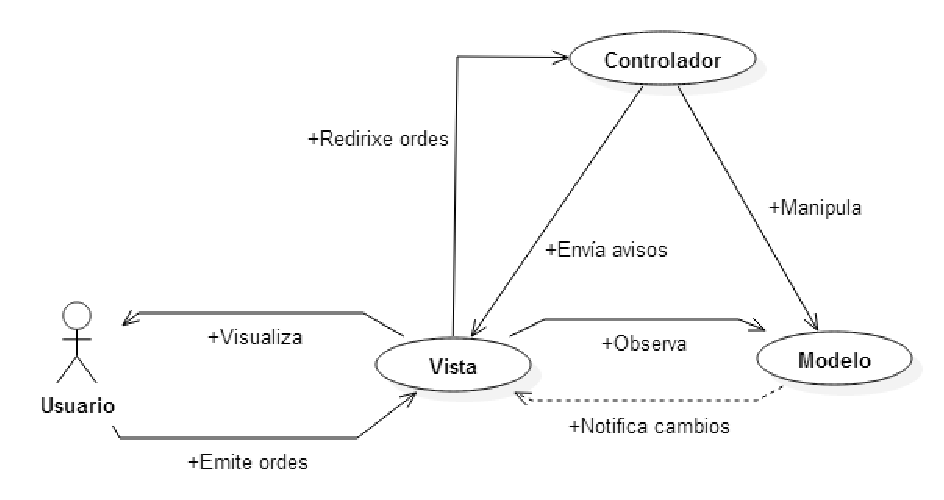
\includegraphics[width=\textwidth,height=\textheight,keepaspectratio]{figuras/MVC}
\caption{Modelo-Vista-Controlador para JDataMotion}
\label{MVC}
\end{figure}

As relacións marcadas cunha liña sólida son asociacións directas (unha clase que actúa de xeito explícito sobre os atributos ou métodos doutra), mentres que a relación marcada cunha liña descontinua representa unha relación indirecta (por exemplo, unha clase que resulta afectada pola actividade doutra). As relacións entre compoñentes detallaranse a continuación.

\begin{itemize}
\item O usuario emite ordes en forma de eventos cara a Vista ao interactuar cos seus botóns e menús.
\item A Vista identifica os eventos que recibe e redirixe cara o Controlador a orde asociada ao evento en cuestión.
\item O Controlador envía un aviso directo á Vista en caso de que a orde que recibe dela levase ao sistema a un estado de erro.
\item O Controlador manipula o Modelo segundo o contido da orde que recibe.
\item O Modelo actúa como entidade observada de cara á Vista. A Vista ten acceso ao Modelo para actualizar a súa aparencia.
\item Do mesmo xeito, que o Modelo sexa observado pola Vista implica que os cambios no modelo serán notificados á Vista, para que esta se actualice no momento do cambio.
\end{itemize} 

Imos documentar máis en profundidade a relación entre a Vista e o Modelo. Comentábamos que a Vista accede ao Modelo para actualizarse cando o desexe, pero ademais o Modelo, cando cambia, notifica á Vista o suceso deste cambio. Temos entón que a Vista actúa como entidade ``observadora'' dun Modelo que é a entidade ``observada''. En esencia, estamos definindo o patrón de deseño Observer.

O patrón de deseño Observer é a mellor resposta que podemos atopar a nivel de deseño para solucionar o problema de manter actualizados ao mesmo nivel o Modelo e a Vista. Se non botásemos man desta solución, teríamos dúas alternativas:

\begin{itemize}
\item Refrescar a vista cada certo intervalo tempo, o cal é ineficiente e seguiría permitindo a posibilidade de que se dese unha incoherencia Vista-Modelo entre refrescos.
\item Permitir ao Modelo que acceda directamente á Vista para invocar un método de actualización, é dicir, asociar directamente a Vista ao Modelo. Isto atenta contra a natureza do Modelo-Vista-Controlador, xa que o Modelo ten que almacenar a información do sistema e abstraerse por completo da Vista ou do módulo que se encargue de representar os seus contidos. Témonos que manter na premisa de que a Vista pode observar ao Modelo e acceder a el para ler datos, pero o Modelo non debe ser consciente da existencia de ningunha Vista.
\end{itemize} 

O patrón Observer pódese aplicar de forma moi sinxela ao noso proxecto. Basta con facer que a Vista implemente a interface \textit{Observer}, de xeito que a obrigue a implementar un método de actualización chamado \textit{update()}, que se disparará cando un obxecto observado cambie o seu estado. Por outra parte, o Modelo só necesita estender a clase \textit{Observable} para ser susceptible de ser observado por un \textit{Observer}. Ao estender esta clase, a Vista xa pode chamar ao método \textit{addObserver(Observer o)} do Modelo, pasándose a ela mesma como parámetro para así incluírse como observadora e ser notificada dos seus cambios.

A asociación dos patróns Modelo-Vista-Controlador e Observer baixo esta forma é bastante común. O libro Pattern-Oriented Software Architecture \cite{pattern-oriented-software-architecture} fai unha boa exposición do que acabamos de mencionar, e aporta o diagrama da figura \ref{MVC-observer} para sintetizar ambos patróns.

\begin{figure}
\centering
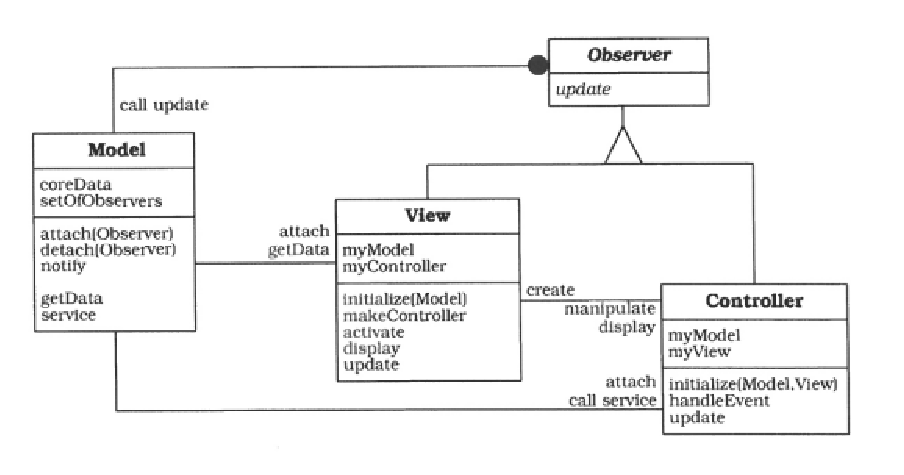
\includegraphics[width=\textwidth,height=\textheight,keepaspectratio]{figuras/MVC-observer}
\caption{Modelo-Vista-Controlador con Observer}
\label{MVC-observer}
\end{figure}

Probablemente a diferencia máis destacable que podemos atopar entre este diagrama e o diagrama que correspondería coa nosa aplicación sería que no noso caso só a Vista implementará a interface \textit{Observer}. O Controlador no noso proxecto non ten que actuar de ningún xeito especial ante os cambios do Modelo, xa que de feito el é o responsable directo deses cambios, e non necesita ser notificado das súas propias accións.